%----------------------------------------------------------------
%
%  File    :  vpn_evaluation.tex
%
%  Author  :  Keith Andrews, IICM, TU Graz, Austria
% 
%  Created :  22 Feb 96
% 
%  Changed :  19 Feb 2004
% 
%----------------------------------------------------------------

\chapter{Evaluation} \label{chap:Evaluation}

In this chapter, we present the results of our model learning and model-based fuzzing. We begin with a discussion and comparison of the various learned models in Section \ref{sec:learnresults} and then move on to presenting the results of our model-based fuzzing in Section \ref{subsec:fuzzresults}.

\section{Learning Results} \label{sec:learnresults}
% section where we show and analyze reference and no filter models including model and statistics
\todo[inline]{rewrite / expand on this portion, detail exact configurations / should I detail it again if I already did so in methods?}
Over the course of our work, we learned a wide variety of different models. In the following, we present the four most relevant ones, all learned from a Linux Strongswan U5.9.5 server, using both the $KV$ and $L^*$ learning algorithms. Error codes have been simplified for better readability. As our \ac{sul} had some issues with non-determinism while retransmissions were enabled, one major differentiating factor in our models is whether retransmission-filtering was enabled for the learning process. This had a significant impact on the resulting learned model, with the version without filtering boasting more than twice the number of states than the one with. Additionally, even when using the methods to combat non-determinism described in Chapter \ref{chap:Learning}, Section \ref{subsec:nondet} the resulting models still occasionally differed when not filtering out retransmissions. Therefore, while still suitable for fingerprinting, the non-filtered models were not used for fuzzing, as we desired a completely deterministic model to serve as our baseline.

\subsection{Learned Models} \label{subsec:models}
Figures \ref{fig:ret_case1} and \ref{fig:ret_case2} show the two most commonly learned models when not filtering retransmissions. Roughly than 80\% of all learning attempts without filtering resulted in one of these two models, which we will refer to as the common models, with the other 20\% being a non-uniform assortment of outliers, an example of which can be seen in Figure \ref{fig:ret_case2}. 

The first common model, presented in Figure \ref{fig:ret_case1} took approximately 52 minutes (3092 seconds) to learn with the $KV$ algorithm, spread over seven learning rounds, and consists of 10 states. Of those 52 minutes, roughly half were used for state exploration / membership queries and the other half for conformance checking, with conformance checking taking slightly longer (1501 vs 1591 seconds). 171 membership queries were performed by the learning algorithm in 2047 steps, whereas 100 equivalence queries were performed for conformance checking in 1826 steps. In contrast, when learned with the $L^*$ algorithm, model learning took almost 85 minutes (5094 seconds) over five learning rounds. Here, the split between state exploration and conformance checking was more distinct, with state exploration taking up approximately 68\% of the total runtime and conformance checking only requiring the remaining 32\% (3489 vs 1605 seconds). Notably, the time needed for conformance checking remained largely the same between the two algorithms, however the difference in state exploration / membership queries is quite large. We discuss this behavior in more detail including a statistical comparison of the two algorithms in Subsection \ref{subsec:comp_kv_lstar}.

Moving on to an examination of the model itself, we can clearly see a separation between the two phases. Phase one completes in state \emph{S3}, and phase two begins right thereafter. While phase one looks very clean and is in fact identical to the model learned with retransmission-filtering enabled, phase two has many strange transitions caused by retransmissions. For example, the transition from state \emph{S5} to \emph{S7} via \emph{sa\_main} returns a valid \emph{IPSEC SA} response. This should be impossible, as phase one messages are ignored while in phase two. However, due to specific timings of retransmissions, this phase one input results happens to be listening for a response when the \ac{sul} sends a retransmission for previous \emph{sa\_quick} message. Next we can see a transition throughout states \emph{S6} to \emph{S11}. In these states, we can see that phase one messages, which are usually ignored in phase two, result in \emph{IPSEC SA} responses. This behavior is caused by retransmissions being treated as responses to phase one messages sent in phase two, which are in fact ignored by the server. Another noticeable property of the learned automata, is that past state \emph{S2}, no paths lead back to the initial state. This is due to the fact that we did not include the delete command in the alphabet for this learned model. Adding delete adds transitions from every state back to the initial one, but also dramatically increases the runtime and non-deterministic behavior of the \ac{sul}, as even more retransmissions are triggered. While not part of our input alphabet, it could be included in future work.

\begin{figure}[ht]
	\centering
	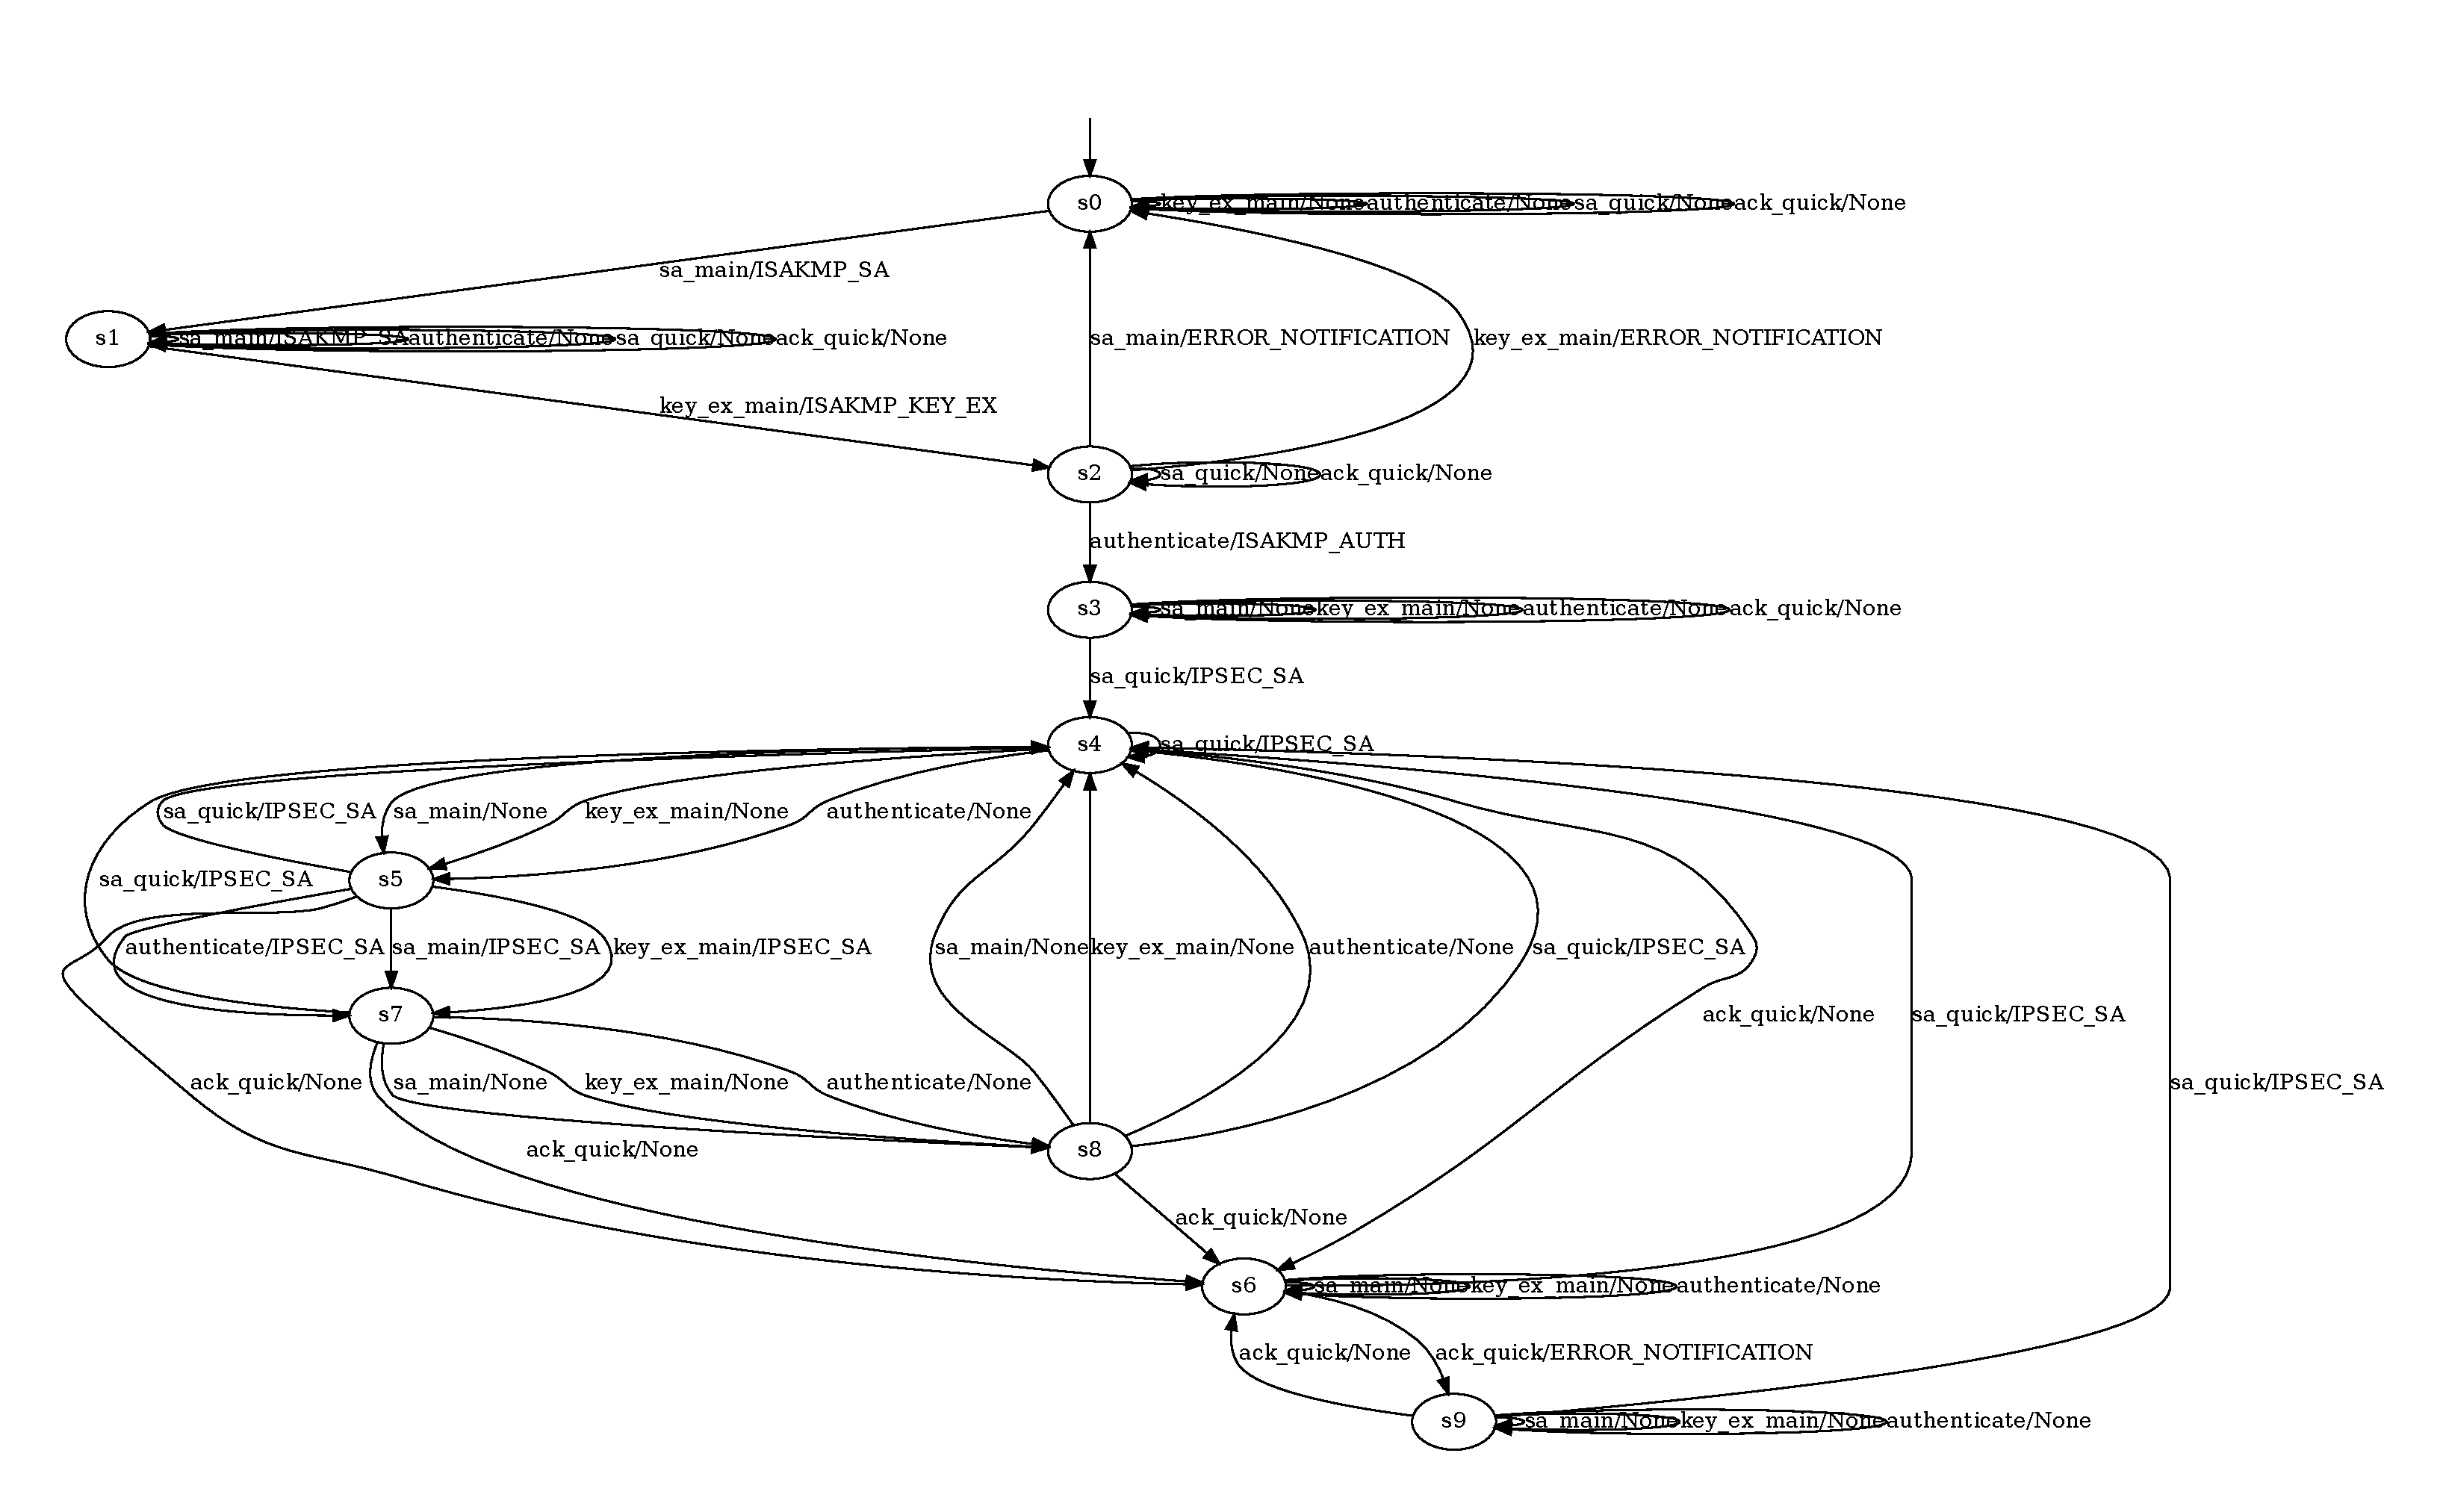
\includegraphics[width=\linewidth]{images/models/retransmissions/retrans_case1}
	\caption{First commonly learned model with retransmissions.}
	\label{fig:ret_case1}
\end{figure}

The second common model, seen in Figure \ref{fig:ret_case2}, took approximately 75 minutes (4507 seconds) to learn using the $KV$ algorithm. The model took nine rounds to learn, and consists of 12 states. Of those 75 minutes, roughly 53\$ were used for state exploration / membership queries and the other 47\% (2382 vs 2126 seconds). 215 membership queries were performed by the learning algorithm in 2219 steps, whereas 120 equivalence queries were performed for conformance checking in 1964 steps. In contrast, when learned with the $L^*$ algorithm, model learning took significantly longer, running for 125 minutes (7520 seconds) over five learning rounds. Here, the split between state exploration and conformance checking was again very distinct, with state exploration taking up approximately 71\% of the total runtime and conformance checking only requiring the remaining 29\% (5393 vs 2126 seconds). Again, the time needed for conformance checking remained largely the same between the two algorithms, however the difference in state exploration / membership queries is even larger.

Examining the model, we can again see a clear separation between the two phases. Phase one for this model is identical to the previous one. Phase two shows a larger number of retransmission-induced strange behavior over the states \emph{S5}, \emph{S7}, \emph{S8}, \emph{S10}, \emph{S11} and \emph{S9}. Again we have phase one inputs, such as \emph{sa\_main}, resulting in the valid phase two output, \emph{IPSEC SA}. This behavior is again triggered by specific timings of retransmissions. Same as in Figure \ref{fig:ret_case1}, no paths past state \emph{S2} lead back to the initial state.

\begin{figure}[hb]
	\centering
	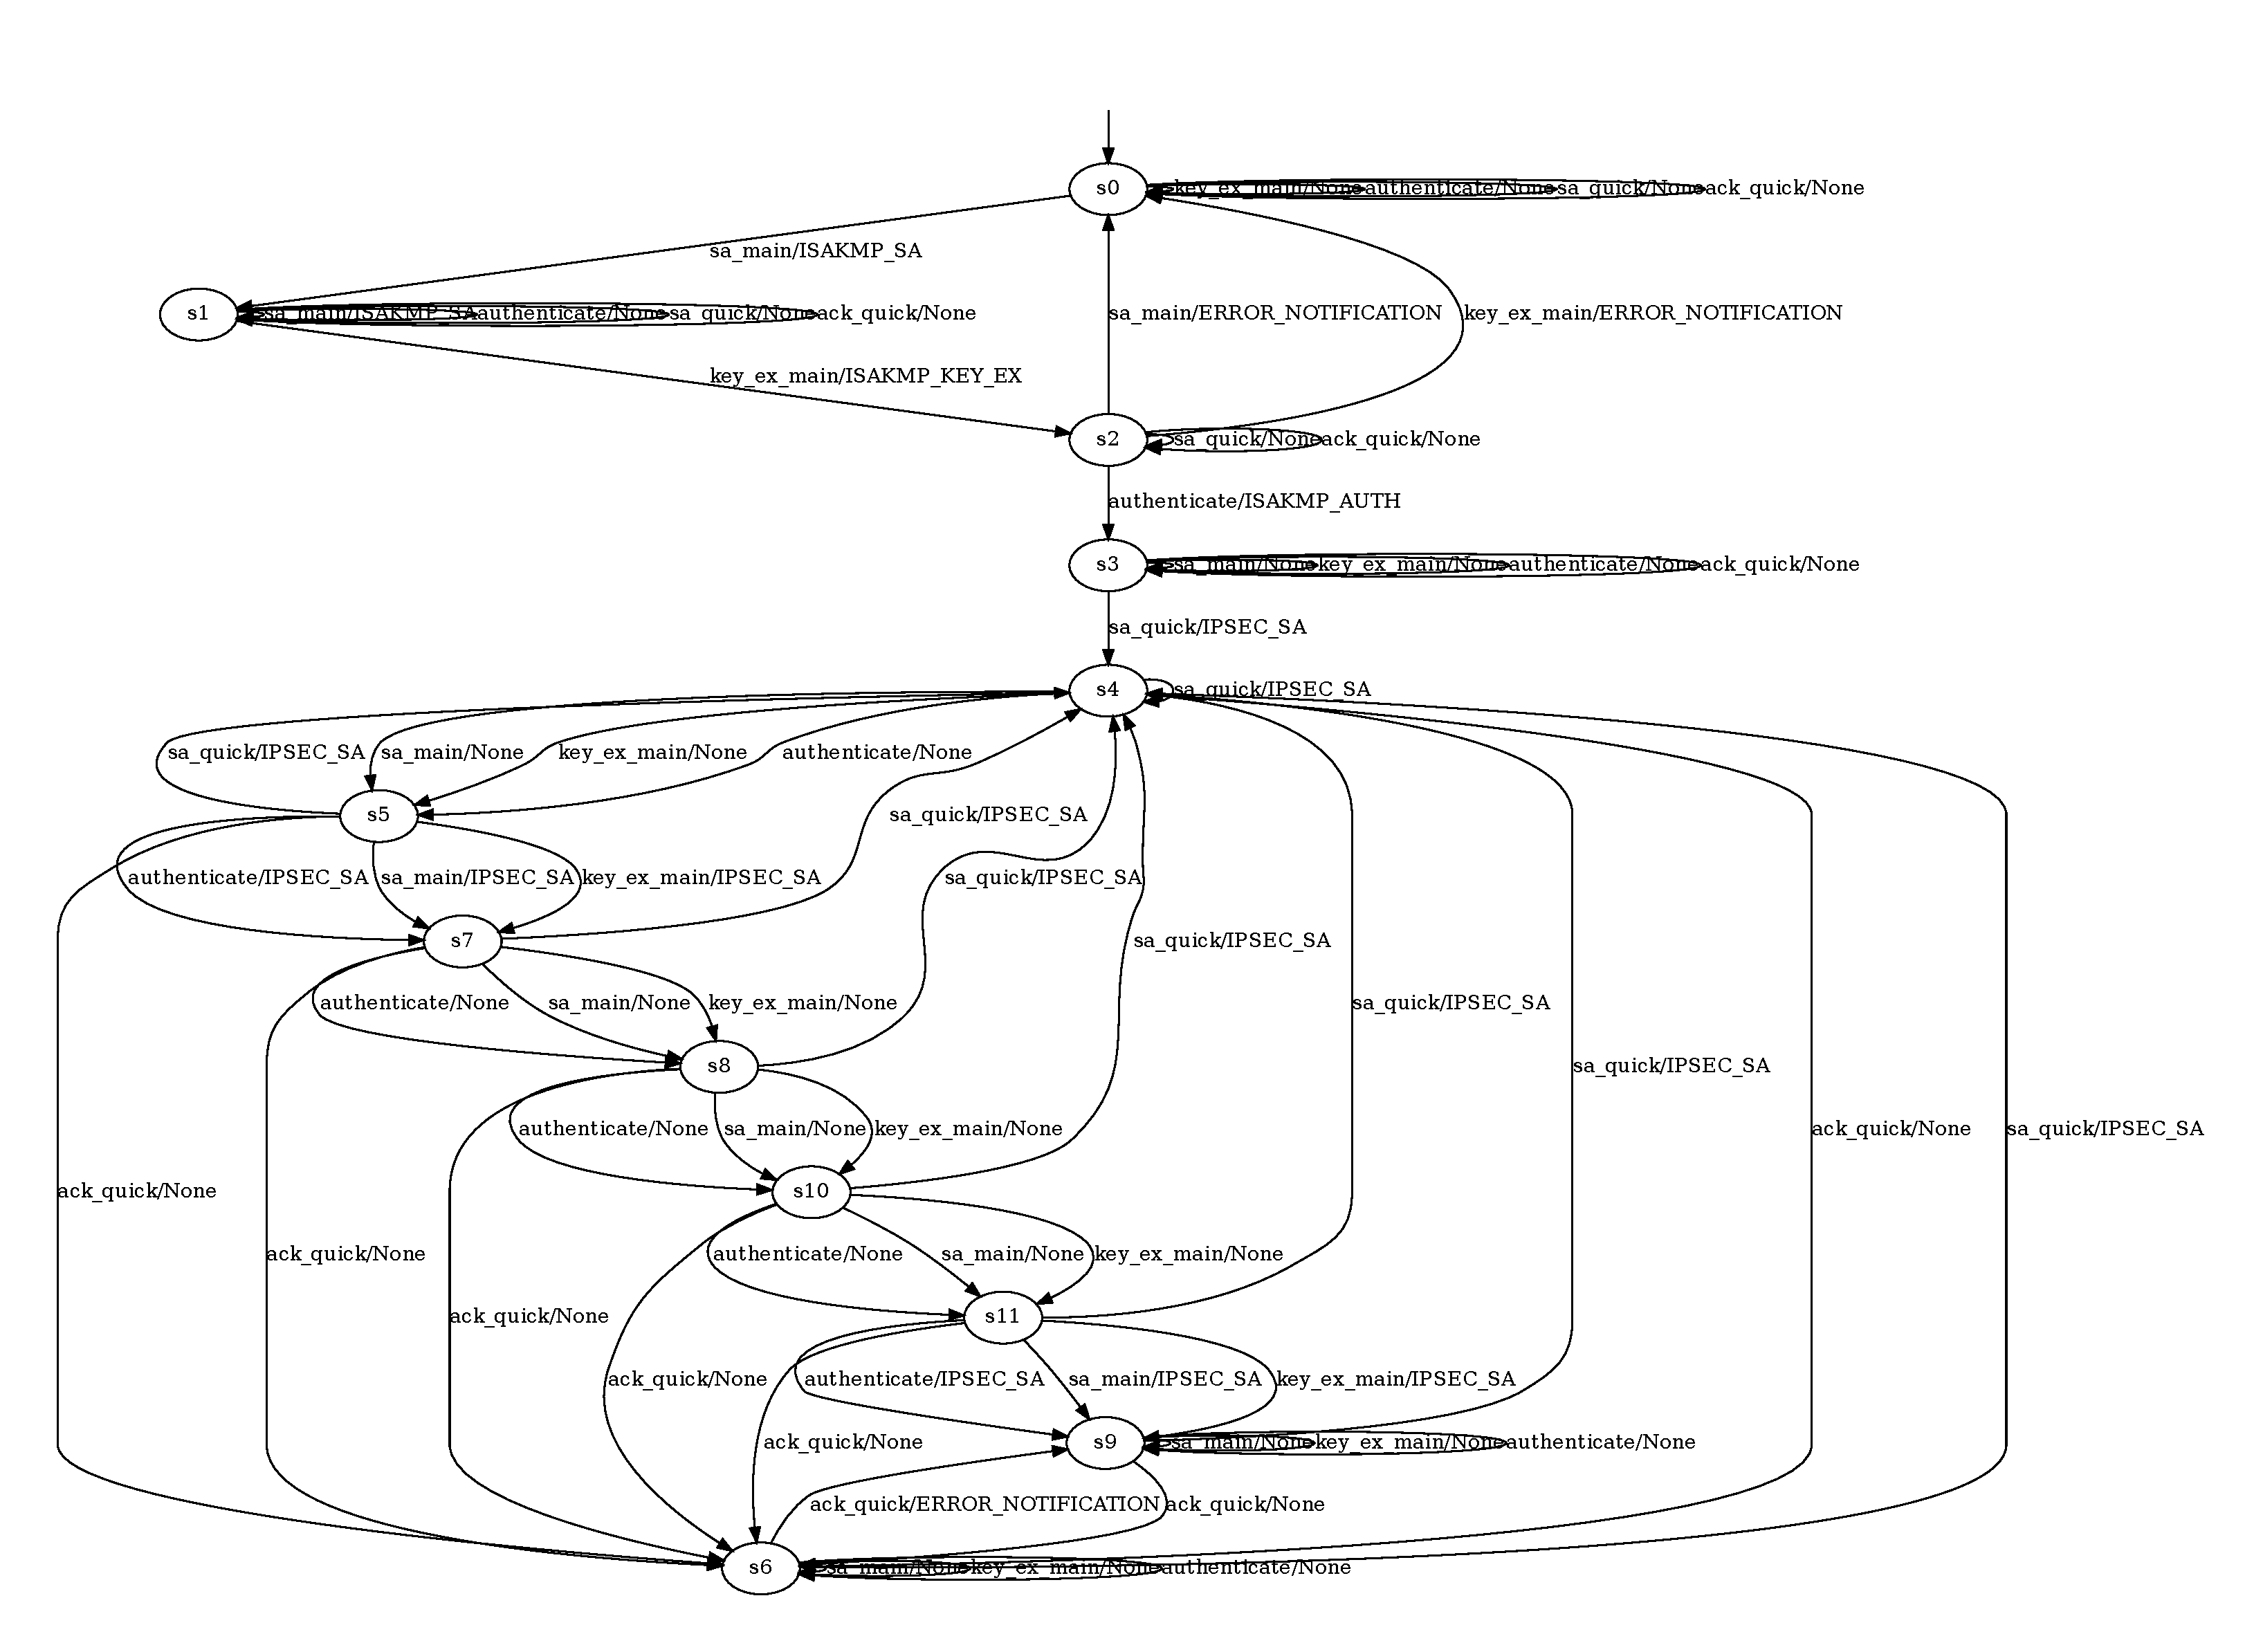
\includegraphics[width=\linewidth]{images/models/retransmissions/retrans_case2}
	\caption{Second commonly learned model with retransmissions.}
	\label{fig:ret_case2}
\end{figure}

In comparison, when learning the same server using retransmission-filtering, all non-deterministic behavior vanishes and we get the model shown in Figure \ref{fig:reference} every learning attempt. The model has only 6 states and therefore was learned much more quickly than the previous ones, with learning requiring only approximately 21 minutes (1266 seconds) using the $KV$ algorithm. Learning happened over four rounds, where the time was distributed between state exploration and conformance checking in a 60-40 split (519 vs 747 seconds). In comparison, when learned with the $L^*$ algorithm, learning took roughly 36 minutes (2157 seconds), spread over two learning rounds. Of that time, state exploration required roughly 55\% compared to the 45\% needed for conformance checking (1188 vs 969 seconds). Compared to $KV$, state exploration / membership queries took more than twice the amount of time to complete.

\begin{figure}[h]
	\centering
	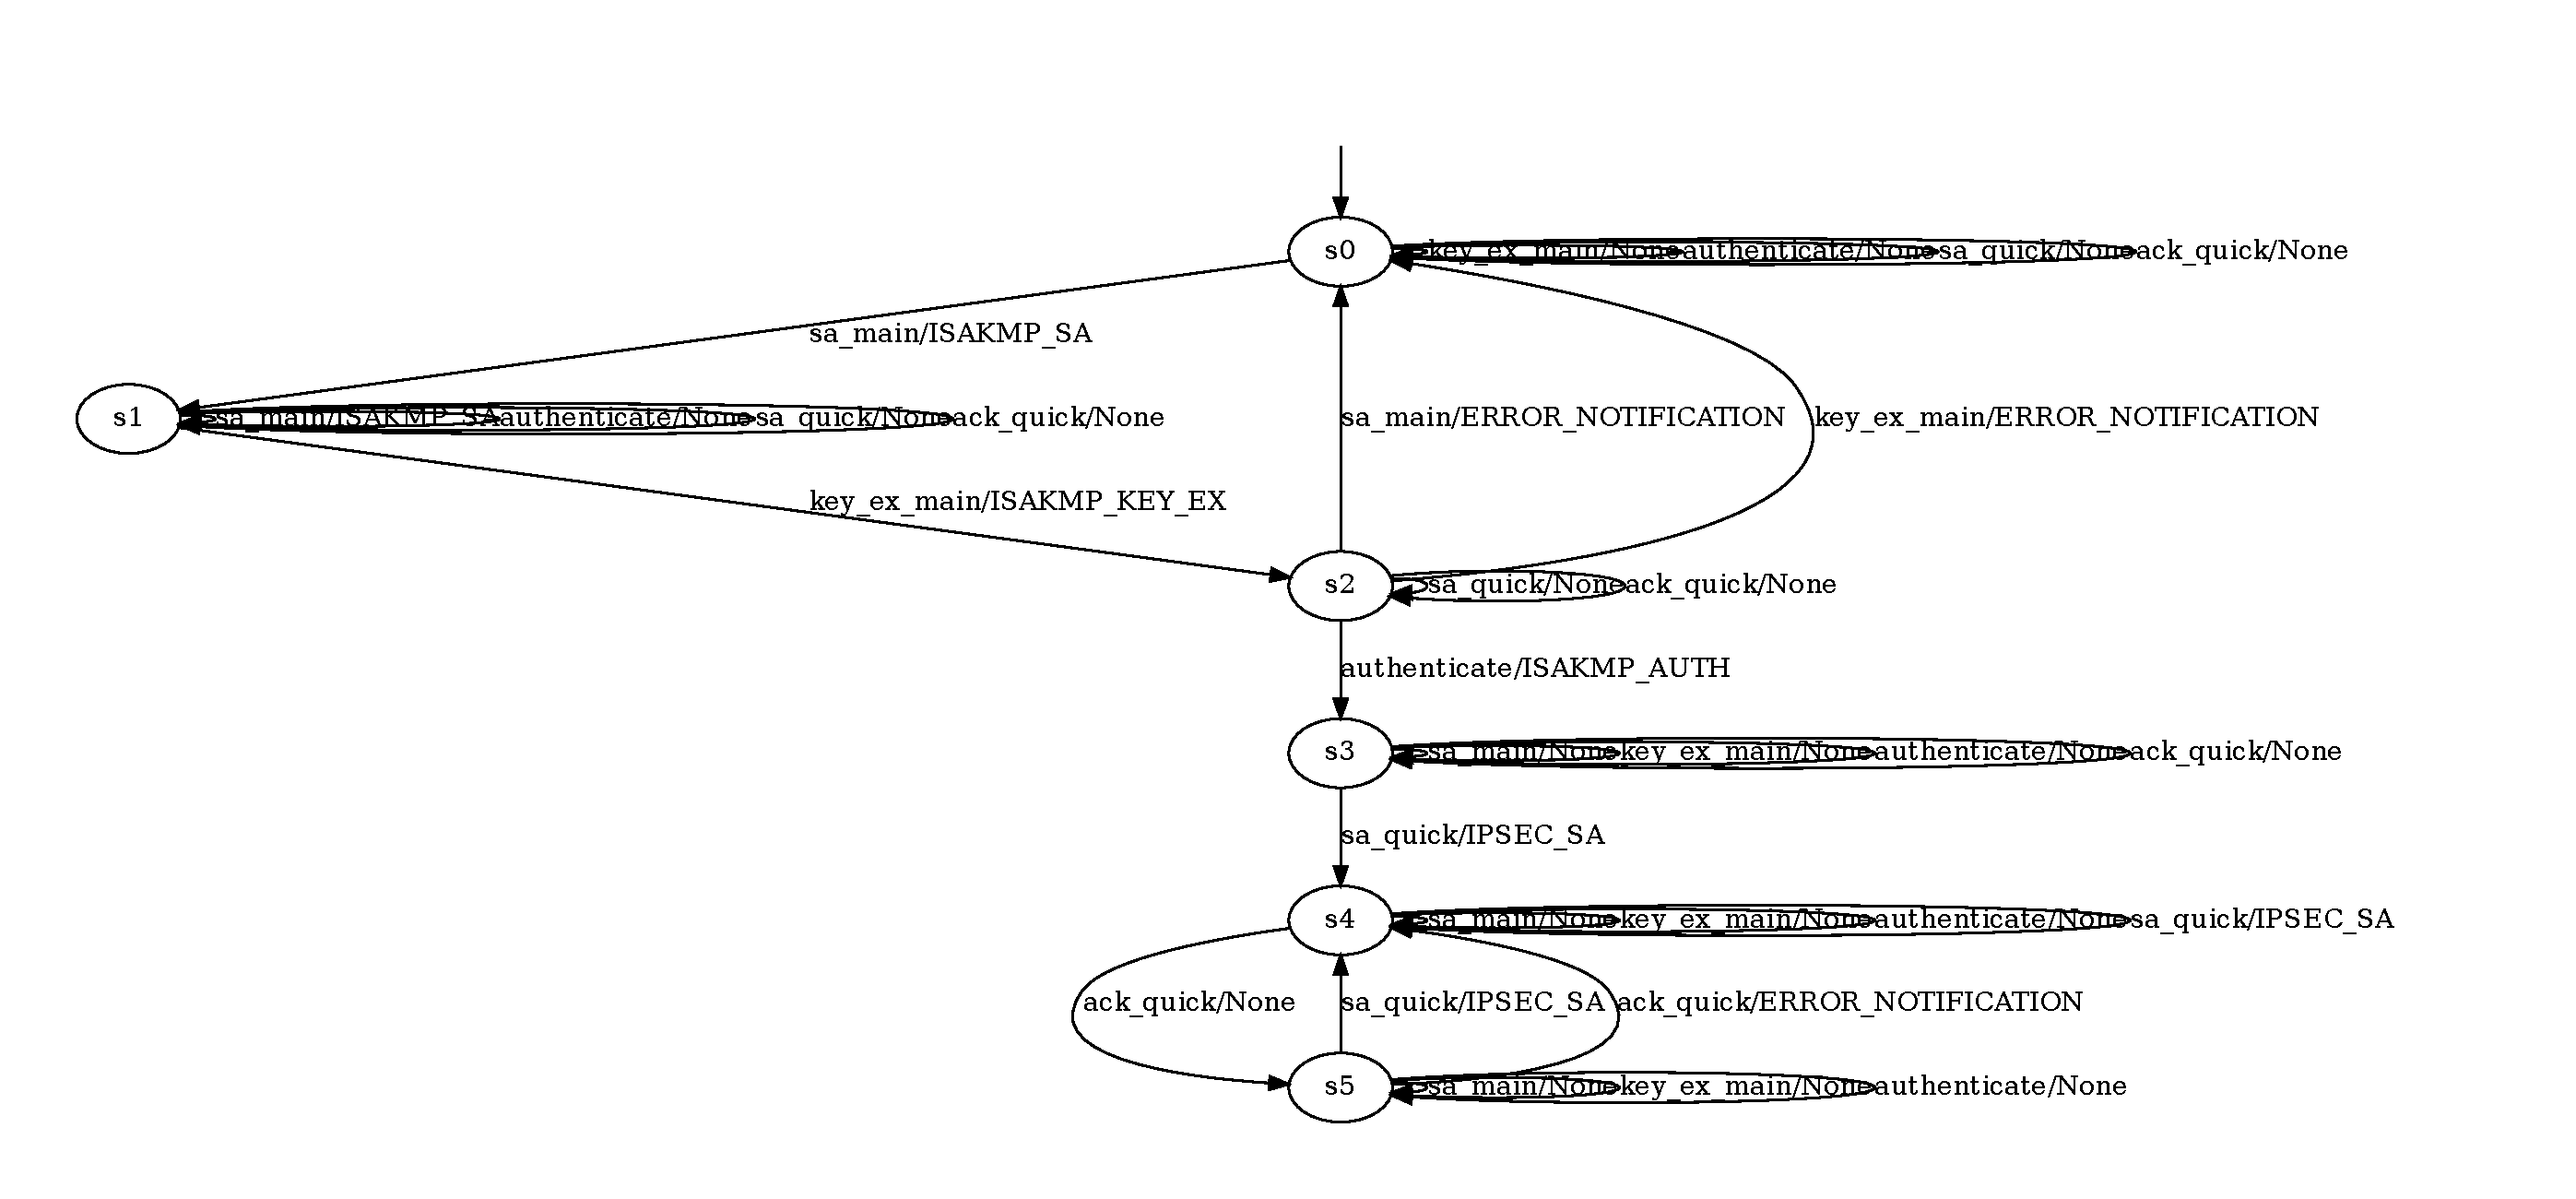
\includegraphics[width=\linewidth]{images/models/Reference}
	\caption{Clean model learned using retransmission filtering}
	\label{fig:reference}
\end{figure} 

Looking at the resulting model more closely, we can see that the first four states are again identical to the previous model. This is due to the fact that the retransmissions only triggered for phase two messages and since they are our only source of non-determinism, we see no differences here. However, the phase two states look wildly different, showing a streamlined behavior that fits our reference \ac{ike} exchange (see Figure \ref{fig:IKEv1}) almost perfectly. The only small difference lies in the additional state \emph{S5} which loops back to state \emph{S4} with an \emph{IPSEC SA} or \emph{ACK} message. This behavior demonstrates how one can create multiple \ac{ipsec} SAs on a single \ac{ike} \ac{sa} channel. And once a new \ac{ipsec} \ac{sa} has been established, we can again send another \emph{ACK} message. In other words, the extra state is there to show that we cannot acknowledge a single \ac{ipsec} \ac{sa} twice, but need to first create a new one.

\todo{stuff here}
% Error model
TODO: analyze error model
Figure \ref{fig:withfilterwitherrors} shows a model learned with retransmission-filtering enabled. Additionally, the input alphabet was expanded to include an additional erroneous version of each letter that maps to a malformed \ac{ike} message. This model served as the basis for our model-based fuzzing and was, thanks to the retransmission-filtering, 100\% deterministic. It took a total of 

TODO: rerun learning with Lstar alg, as runtime seems sus

The model looks largely identical to the previous model, apart from some additional self-transitions and one additional error transition from state \emph{S4} to \emph{S5}. Here, state \emph{S4} corresponds to the previous \emph{S6}. The error transition simply means that we need to create a valid \ac{ipsec} \ac{sa} before we can acknowledge it.

\begin{figure}
	\centering
	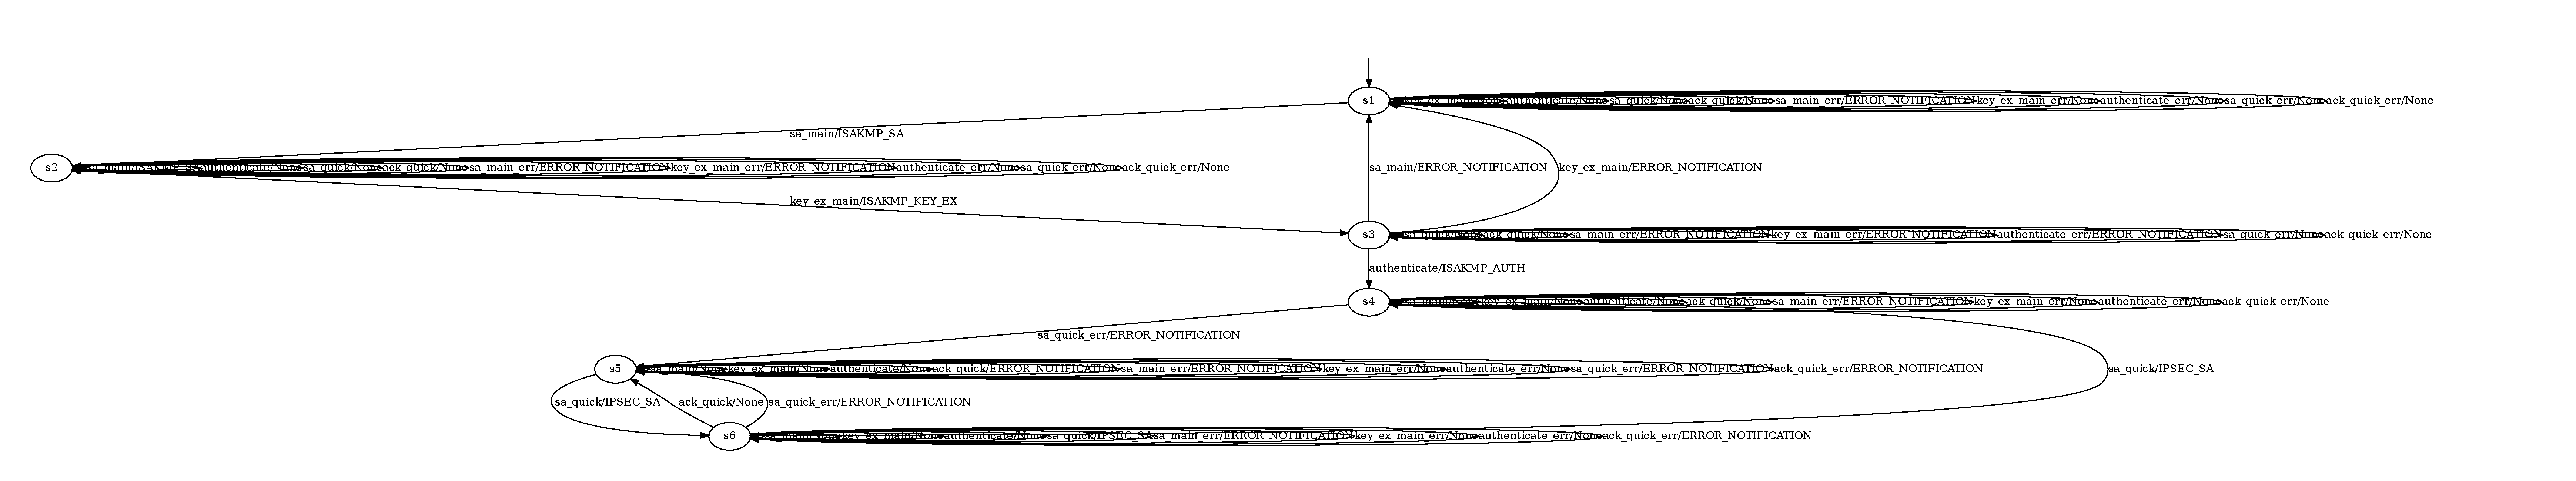
\includegraphics[width=\linewidth]{images/models/WithFilterWithErrors_kv}
	\caption{Model with malformed messages}
	\label{fig:withfilterwitherrors}
\end{figure}

\subsection{Comparing $KV$ and $L^*$} \label{subsec:comp_kv_lstar}
% section copmaring KV and Lstar
Table \ref{tab:compkvlstar} shows average performance statistics over five learning runs each, with retransmission-filtering enabled. The same hardware and software configurations were used as described in Chapter \ref{sec:learnenv} with the learning program set up on a VirtualBox 6.1 \ac{vm} allotted 4GB of memory and one CPU core. We used all the basic packets for our input alphabet, so
\emph{sa\_main}, \emph{key\_ex\_main}, \emph{authenticate}, \emph{sa\_quick} and \emph{ack\_quick}. The model learned is the clean model seen in Figure \ref{fig:reference}. Table \ref{tab:compkvlstar} shows the metric on the left and the respective averages for the $L^*$ and $KV$ learning algorithms respectively on the right. Interesting results are highlighted in bold. From top to bottom, the metrics measured are as follows.
Learning rounds refers to the number of rounds the learning algorithms had to run for, or in other words, how many attempts they needed to correctly learn the \ac{sul}. Total time is the total time needed by the algorithm from start to the finished model. The total time can be split into time spent on the learning algorithm and time spent on equivalence queries. Learning membership queries refers to the number of membership queries sent to the SUL while learning steps to the steps in the learning algorithm itself. Analogously, equivalence oracle queries refers to the equivalence queries sent to the SUL and equivalence oracle steps to the steps needed by the equivalence oracle implementation. Finally, membership queries saved by caching details the performance boost gained by caching membership queries, with the value indicating the number of queries saved.

As the only difference between the two configurations tested was the choice of learning algorithm, intuitively we expect relevant fields to vary the most with equivalence oracle field to be largely unchanged. This intuition is confirmed by our experiments, wherein while the time spent on equivalence queries was very similar, the time spent on membership queries differed greatly. The $L^*$ algorithm required more than double the number of membership queries than its $KV$ counterpart. As membership queries are the main performance bottleneck in our setup, this change of course led to a significantly better runtime for $KV$, with total time spent on the learning algorithm being close to half that of the $L^*$ algorithm. This difference in time spent on the learning algorithm meant, that for this experiment, the $KV$ algorithm learned a model in roughly 75\% of the time needed by the $L^*$ algorithm. Looking only at the learning algorithm, $KV$ performed roughly twice as well as its counterpart.

Little variance was observed throughout previous learning attempts so this small sample size is believed to be representative. However, for even more accurate results the experiment should be carried out again for more runs. 

\todo{Redo with results from 20 runs. And detail standard deviation and such statistics.}

\begin{table}[t]
	\centering
	\begin{tabular}{ |p{6.5cm}||p{1cm}|p{1cm}|  }
		\hline
		\multicolumn{3}{|c|}{\textbf{Learning Algorithm Performance (Averages)}} \\
		\hline
		\textbf{Metric} & $\mathbf{L^*}$ & $\mathbf{KV}$ \\
		\hline
		Learning Rounds							&	2				&	4 				\\
		Total Time (s)							&   3036			& 	2296   			\\
		Time Learning Algorithm	(s)				&	\textbf{1624}	& 	\textbf{879}	\\
		Time Equivalence Checks (s)				& 	1412			& 	1417			\\
		Learning Membership Queries 			&   \textbf{177}	& 	\textbf{79}		\\
		Learning Steps							& 	867	  			& 	753   			\\
		Equivalence Oracle Queries				& 	60  			&  	60				\\
		Equivalence Oracle Steps				& 	748  			&  	991				\\
		Membership Queries Saved by Caching		& 	14  			&  	27				\\
		\hline
	\end{tabular}
	\caption{Comparison $L^*$ and $KV$}
	\label{tab:compkvlstar}
\end{table}

\subsection{Library Error} \label{subsec:liberror}
% section with discovered bug
Another notable finding from the model learning phase, was the discovery of a bug in a used Python Diffie-Hellman key exchange library. The bug was only found thanks to the exhaustive number of packets sent with our mapper class and due to the non-determinism checks implemented in \textsc{AALpy}. Despite our best efforts in removing the non-deterministic behavior from our learning process, we would still get occasional non-determinism errors at random points while learning. This problem persisted over several weeks due to the fact that the errors occurred randomly and only sporadically during some learning attempts. Initially we believed this to be also caused by retransmissions, but since the problems persisted even after introducing retransmission-filtering, that possibility was ruled out. The other option was of course problems in our implementation of the \ac{ipsec} protocol. Therefore, a lot of time was invested into painstakingly comparing logs and packet captures between our implementation and the \ac{sul} to ensure that everything lined up, since \textsc{AALpy} was still reporting non-determinism errors. Finally we discovered a discrepancy between the two and through it, that the problems were not in fact caused by our implementation, but by a used Python library. It turns out there was a very niche bug in a used Diffie-Hellman Python library where, if the most significant byte was a zero, it would be omitted from the response, causing the local result to be one byte shorter than the value calculated by the \ac{sul}. As this would only occur in the rare case where the MSB of the DH exchange was zero, this explains the random and difficult to reproduce nature of the bug. This behavior was undocumented and happened in a function call that allowed specifying the length of the returned key. As the library is not a very widespread one, the impact of this bug is presumably not very high. Regardless, it could compromise the security of affected systems and therefore the maintainer of the library has been notified of the problem. Due to the elusive nature of this bug, it would very likely not have been noticed without the exhaustive communication done by the model learning process and without seeing the slight differences in the resulting models that did not crash during the learning process.

\section{Fuzzing Results} \label{subsec:fuzzresults}
\todo[inline]{Fuzzing results}
\todo[inline]{Compare mutation based fuzzing and filtering results / runtimes}